\section{Solution Design}
\label{sec:approach:solution}

Based on the constraints and definitions shown in Section \ref{sec:approach:def}, an offline system for EAM learning is presented. The inputs of the learning system are:

\begin{enumerate}
 \item Context knowledge: the context knowledge represents the prior knowledge provided by a domain expert and which is relevant to learn activity models. The concepts modelled in the context knowledge include: 
 \begin{enumerate}
  \item Activities: type, location and IAM
  \item Objects: type, location and attached sensors
  \item Sensors: type, described action and object to which it is attached
 \end{enumerate}
 
 \item Sensor activation dataset: an unlabelled time-stamped sensor activation dataset with the activity traces of a concrete user.
\end{enumerate}

In the current implementation, context knowledge is formatted in a \textit{Json}\footnote{http://json.org/} file. As an example, Figure \ref{fig-context-json} shows how an activity, an object and a sensor are modelled in the context knowledge file. This knowledge is provided by a domain expert and modelled by knowledge engineers. Sensor activation datasets are formatted in Comma Separated Value files (CSV). Each row of the file contains a time-stamp (year, month, day and time) and a sensor activation (see Figure \ref{fig-dataset}).

\begin{figure}[htbp]
\begin{small}
\begin{lstlisting}
"MakeCoffee": {
	"type": ["Cooking"],
	"location": ["Kitchen"],
	"IAM": ["hasContainer", "hasCoffee"],
	"duration": 300
}
---------------------------------------------------
"kitchen-tap": {
	"type": ["Cooking", "HouseWork"]
	"location": "Kitchen"
	"sensors": ["ktapSens"]
}
---------------------------------------------------
"ktapSens": {
	"type": "tilt",
	"action": "turnOnTap",
	"attached-to": "kitchen-tap"
}
\end{lstlisting}
\end{small}
\caption{Example of activities, objects and sensors modelled in the context knowledge file. Activity duration is given in seconds.}
\label{fig-context-json}
\end{figure}

\begin{figure}[htbp]
\begin{small}
\begin{lstlisting}
2014-05-23 09:47:33.984341,storeSens
2014-05-23 09:47:39.333528,potSens
2014-05-23 09:47:52.750216,cookerSens
2014-05-23 09:48:07.764138,fridgeSens
2014-05-23 09:48:12.591836,wmilkSens
2014-05-23 09:48:47.199512,chocoSens
2014-05-23 09:54:11.553695,mugSens
2014-05-23 09:54:40.794979,rcontrolSens
2014-05-23 09:54:50.390696,tvSens
2014-05-23 09:54:59.348862,sofaSens
\end{lstlisting}
\end{small}
\caption{A slice of a sensor activation dataset.}
\label{fig-dataset}
\end{figure}

Based on those inputs, the output of the presented approach is a list of action sequences for each activity, which describe the EAMs for each activity (see equation \ref{eq-eam}). %To learn those models a two-step system is presented. First, a clustering process is run in the so called \textbf{semantic space of actions}, using initial activity models to label each cluster with a modeled activity. The semantic space of actions is a three-dimensional space spanned by the axes of location, type and time. Actions carried out by a user have only one location in the environment (bathroom, kitchen etc.), one time instant, but multiple types. For instance, a glass can be used for multiple activity types, such as cooking, eating or personal hygiene (brushing teeth). Hence, the action \textit{hasContainer} linked to a glass activation, occupies multiple positions in the type axis. 

The designed system architecture to learn EAMs is depicted in Figure \ref{fig-design}. All the modules of the diagram have been implemented using Python 2.7\footnote{https://www.python.org/} and its packages Numpy\footnote{http://www.numpy.org/} for numerical computing and Pandas\footnote{http://pandas.pydata.org/} for data analysis. 

Firstly, a sensor activation dataset has to be collected. A real smart environment or a synthetic data generator can be used to get this dataset. Afterwards, a novel clustering process is run, using the context knowledge provided by an expert. The clustering process is divided into two steps: (i) the Semantic Activity Annotation algorithm ($SA^3$) uses IAMs to detect activities in the unlabelled dataset and initialise activity clusters, and (ii) the Activity Clustering algorithm ($AC$) uses activity, object and action knowledge to expand initial activity clusters detected by $SA^3$. As a result, several action clusters for every activity are generated. Those clusters are finally processed by Activity Model Learner ($AML$), which filters incorrect action sequences and outliers to learn final EAMs as a list of action sequences.

%Firstly, a sensor activation dataset has to be collected. A real smart environment or a synthetic data generator can be used to get this dataset. Afterwards, a novel clustering process is run, using the context knowledge described in a \textit{Json}\footnote{http://www.json.org/} file. The clustering process is divided into two steps: (i) the Semantic Activity Annotation algorithm ($SA^3$) uses IAMs to detect activities in the unlabeled dataset and initialize activity clusters, and (ii) the Activity Clustering algorithm ($AC$) uses activity, object and action knowledge to expand initial activity clusters detected by $SA^3$. As a result, several action clusters for every activity are generated. Those clusters, stored in another \textit{Json} file, are finally processed by Activity Model Learner, which filters incorrect action sequences and outliers to learn final EAMs as a list of action sequences.

\begin{figure}[htbp]
\centering
\includegraphics[width=\textwidth]{our_approach.pdf}
    \caption{The detailed design architecture of the proposed approach.}
    \label{fig-design}
\end{figure}